<!-- Generated by pkgdown: do not edit by hand -->
<!DOCTYPE html>
<html lang="en">
  <head>
  <meta charset="utf-8">
<meta http-equiv="X-UA-Compatible" content="IE=edge">
<meta name="viewport" content="width=device-width, initial-scale=1.0">

<title>IBMPopSim C++ essentials • IBMPopSim</title>


<!-- jquery -->
<script src="https://cdnjs.cloudflare.com/ajax/libs/jquery/3.4.1/jquery.min.js" integrity="sha256-CSXorXvZcTkaix6Yvo6HppcZGetbYMGWSFlBw8HfCJo=" crossorigin="anonymous"></script>
<!-- Bootstrap -->
<link href="https://cdnjs.cloudflare.com/ajax/libs/bootswatch/3.4.0/cosmo/bootstrap.min.css" rel="stylesheet" crossorigin="anonymous" />


<script src="https://cdnjs.cloudflare.com/ajax/libs/twitter-bootstrap/3.4.1/js/bootstrap.min.js" integrity="sha256-nuL8/2cJ5NDSSwnKD8VqreErSWHtnEP9E7AySL+1ev4=" crossorigin="anonymous"></script>

<!-- bootstrap-toc -->
<link rel="stylesheet" href="../bootstrap-toc.css">
<script src="../bootstrap-toc.js"></script>

<!-- Font Awesome icons -->
<link rel="stylesheet" href="https://cdnjs.cloudflare.com/ajax/libs/font-awesome/5.12.1/css/all.min.css" integrity="sha256-mmgLkCYLUQbXn0B1SRqzHar6dCnv9oZFPEC1g1cwlkk=" crossorigin="anonymous" />
<link rel="stylesheet" href="https://cdnjs.cloudflare.com/ajax/libs/font-awesome/5.12.1/css/v4-shims.min.css" integrity="sha256-wZjR52fzng1pJHwx4aV2AO3yyTOXrcDW7jBpJtTwVxw=" crossorigin="anonymous" />

<!-- clipboard.js -->
<script src="https://cdnjs.cloudflare.com/ajax/libs/clipboard.js/2.0.6/clipboard.min.js" integrity="sha256-inc5kl9MA1hkeYUt+EC3BhlIgyp/2jDIyBLS6k3UxPI=" crossorigin="anonymous"></script>

<!-- headroom.js -->
<script src="https://cdnjs.cloudflare.com/ajax/libs/headroom/0.11.0/headroom.min.js" integrity="sha256-AsUX4SJE1+yuDu5+mAVzJbuYNPHj/WroHuZ8Ir/CkE0=" crossorigin="anonymous"></script>
<script src="https://cdnjs.cloudflare.com/ajax/libs/headroom/0.11.0/jQuery.headroom.min.js" integrity="sha256-ZX/yNShbjqsohH1k95liqY9Gd8uOiE1S4vZc+9KQ1K4=" crossorigin="anonymous"></script>

<!-- pkgdown -->
<link href="../pkgdown.css" rel="stylesheet">
<script src="../pkgdown.js"></script>




<meta property="og:title" content="IBMPopSim C++ essentials" />
<meta property="og:description" content="IBMPopSim" />




<!-- mathjax -->
<script src="https://cdnjs.cloudflare.com/ajax/libs/mathjax/2.7.5/MathJax.js" integrity="sha256-nvJJv9wWKEm88qvoQl9ekL2J+k/RWIsaSScxxlsrv8k=" crossorigin="anonymous"></script>
<script src="https://cdnjs.cloudflare.com/ajax/libs/mathjax/2.7.5/config/TeX-AMS-MML_HTMLorMML.js" integrity="sha256-84DKXVJXs0/F8OTMzX4UR909+jtl4G7SPypPavF+GfA=" crossorigin="anonymous"></script>

<!--[if lt IE 9]>
<script src="https://oss.maxcdn.com/html5shiv/3.7.3/html5shiv.min.js"></script>
<script src="https://oss.maxcdn.com/respond/1.4.2/respond.min.js"></script>
<![endif]-->



  </head>

  <body data-spy="scroll" data-target="#toc">
    <div class="container template-article">
      <header>
      <div class="navbar navbar-default navbar-fixed-top" role="navigation">
  <div class="container">
    <div class="navbar-header">
      <button type="button" class="navbar-toggle collapsed" data-toggle="collapse" data-target="#navbar" aria-expanded="false">
        <span class="sr-only">Toggle navigation</span>
        <span class="icon-bar"></span>
        <span class="icon-bar"></span>
        <span class="icon-bar"></span>
      </button>
      <span class="navbar-brand">
        <a class="navbar-link" href="../index.html">IBMPopSim</a>
        <span class="version label label-default" data-toggle="tooltip" data-placement="bottom" title="Released version">0.3.0</span>
      </span>
    </div>

    <div id="navbar" class="navbar-collapse collapse">
      <ul class="nav navbar-nav">
        <li>
  <a href="../index.html">
    <span class="fas fa fas fa-home fa-lg"></span>
     
  </a>
</li>
<li>
  <a href="../articles/IBMPopSim.html">Get started</a>
</li>
<li>
  <a href="../reference/index.html">Reference</a>
</li>
<li>
  <a href="../articles/IBMPopSim_cpp.html">C++ essentials</a>
</li>
<li class="dropdown">
  <a href="#" class="dropdown-toggle" data-toggle="dropdown" role="button" aria-expanded="false">
    Vignettes
     
    <span class="caret"></span>
  </a>
  <ul class="dropdown-menu" role="menu">
    <li>
      <a href="../articles/IBMPopSim_human_pop.html">Human population</a>
    </li>
    <li>
      <a href="../articles/IBMPopSim_human_pop_IMD.html">Human population with swap</a>
    </li>
    <li>
      <a href="../articles/IBMPopSim_insurance_portfolio.html">Insurance portfolio</a>
    </li>
    <li>
      <a href="../articles/IBMPopSim_interaction.html">Population with genetically variable traits</a>
    </li>
  </ul>
</li>
      </ul>
      <ul class="nav navbar-nav navbar-right">
        <li>
  <a href="https://github.com/DaphneGiorgi/IBMPopSim/">
    <span class="fab fa fab fa-github fa-lg"></span>
     
  </a>
</li>
      </ul>
      
    </div><!--/.nav-collapse -->
  </div><!--/.container -->
</div><!--/.navbar -->

      

      </header>


<div class="row">
  <div class="col-md-9 contents">
    <div class="page-header toc-ignore">
      <h1 data-toc-skip>IBMPopSim C++ essentials</h1>
                        <h4 class="author">Daphné Giorgi, Sarah Kaakai, Vincent Lemaire</h4>
            
      
      <small class="dont-index">Source: <a href='https://github.com/DaphneGiorgi/IBMPopSim/blob/master/vignettes/IBMPopSim_cpp.Rmd'><code>vignettes/IBMPopSim_cpp.Rmd</code></a></small>
      <div class="hidden name"><code>IBMPopSim_cpp.Rmd</code></div>

    </div>

    
    
The arguments \texttt{intensity\_code}, \texttt{interaction\_code} and \texttt{kernel\_code} of the events functions must contain some C++ code given by the user. You don't need to be a C++ guru to write the few instructions needed. These functions should use very little C++ syntax. They are essentially arithmetic or logical operations, tests and calls to predefined functions, which we give an overview below.

For code efficiency, you should not allocate memory in these functions (no \texttt{new}) or use type containers (\texttt{std::vector}, \texttt{std::list}, \ldots). If you think you need to allocate memory, consider as parameter an R vector that will be mapped via \texttt{arma::vector} (see below), or declare the variable as \texttt{static}.
Also, it should not be necessary to make a loop. Keep in mind that these functions should be fast.

There are no C++ language restrictions so you can use all the functions of the standard C++11 library. However we detail in this section some functions that should be sufficient. For more details on C++ and Rcpp we recommend:

\begin{itemize}
\tightlist
\item
  \href{https://www.cplusplus.com/doc/tutorial/}{C++ tutorial}
\item
  \href{http://dirk.eddelbuettel.com/code/rcpp.html}{Rcpp} and \href{http://dirk.eddelbuettel.com/code/rcpp.armadillo.html}{RcppArmadillo}
\item
  \href{https://teuder.github.io/rcpp4everyone_en/}{Rcpp for everyone}
\end{itemize}

\hypertarget{c-syntax}{%
\subsection{C++ syntax}\label{c-syntax}}

\begin{itemize}
\tightlist
\item
  Each statement must be ended by a semicolon.
\item
  Single-line comments start with two forward slashes \texttt{//}.
\item
  To create a variable, you must specify the type and assign it a value (type variable = value;). Here some examples:
\end{itemize}

\begin{verbatim}
int myNum = 5;               // Integer (whole number without decimals)
double myFloatNum = 5.99;    // Floating point number (with decimals)
char myLetter = 'D';         // Character
bool myBoolean = true;       // Boolean (true or false)
\end{verbatim}

\begin{itemize}
\tightlist
\item
  \texttt{bool} data type can take the values \texttt{true} (1) or \texttt{false} (0).
\item
  C++ supports the usual logical conditions from mathematics:

  \begin{itemize}
  \tightlist
  \item
    Less than: \texttt{a\ \textless{}\ b}
  \item
    Less than or equal to: \texttt{a\ \textless{}=\ b}
  \item
    Greater than: \texttt{a\ \textgreater{}\ b}
  \item
    Greater than or equal to: \texttt{a\ \textgreater{}=\ b}
  \item
    Equal to \texttt{a\ ==\ b}
  \item
    Not Equal to: \texttt{a\ !=\ b}
  \end{itemize}
\item
  The logical operators are: \texttt{!}, \texttt{\&\&}, \texttt{\textbar{}\textbar{}}
\item
  The arithmetic operators are: \texttt{+}, \texttt{-}, \texttt{*}, \texttt{/}, \texttt{\%}
\item
  Compound assignment: \texttt{+=}, \texttt{-=}, \texttt{*=}, \texttt{/=}, \texttt{\%=}
\item
  Increment and decrement: \texttt{++}, \texttt{-\/-}
\item
  Conditional ternary operator: \texttt{?\ :}
  The conditional operator evaluates an expression, returning one value if that expression evaluates to \texttt{true}, and a different one if the expression evaluates as \texttt{false}. Its syntax is:
\end{itemize}

\begin{verbatim}
condition ? result1; : result2;
\end{verbatim}

\begin{itemize}
\tightlist
\item
  Use the \texttt{if}, \texttt{else\ if}, \texttt{else} statements to specify a block of C++ code to be executed if one or more conditions are or not \texttt{true}.
\end{itemize}

\begin{verbatim}
if (condition1) {
  // block of code to be executed if condition1 is true
} else if (condition2) {
  // block of code to be executed if the condition1 is false and condition2 is true
} else {
  // block of code to be executed if the condition1 is false and condition2 is false
}
\end{verbatim}

\begin{itemize}
\tightlist
\item
  The syntax of the switch statement is a bit peculiar. Its purpose is to check for a value among a number of possible constant expressions. It is something similar to concatenating \texttt{if-else} statements, but limited to constant expressions. Its most typical syntax is:
\end{itemize}

\begin{verbatim}
switch (expression)
{
  case constant1:
     group-of-statements-1;
     break;
  case constant2:
     group-of-statements-2;
     break;
  .
  .
  .
  default:
     default-group-of-statements
}
\end{verbatim}

It works in the following way: switch evaluates expression and checks if it is equivalent to \texttt{constant1}; if it is, it executes \texttt{group-of-statements-1} until it finds the \texttt{break} statement. When it finds this break statement, the program jumps to the end of the entire switch statement (the closing brace).

\begin{itemize}
\tightlist
\item
  When you know exactly how many times you want to loop through a block of code, use the \texttt{for} loop.
\end{itemize}

\begin{verbatim}
for (statement 1; statement 2; statement 3) {
  // code block to be executed
}
\end{verbatim}

\begin{itemize}
\tightlist
\item
  The while loop loops through a block of code as long as a specified condition is true.
\end{itemize}

\begin{verbatim}
while (condition) {
  // code block to be executed
}
\end{verbatim}

For more details we recommend a few pages of \href{https://www.cplusplus.com/}{www.cplusplus.com} about:

\begin{itemize}
\tightlist
\item
  \href{https://www.cplusplus.com/doc/tutorial/variables/}{Variables}
\item
  \href{https://www.cplusplus.com/doc/tutorial/operators/}{Operators}
\item
  \href{https://www.cplusplus.com/doc/tutorial/control/}{Statements}
\end{itemize}

\hypertarget{usual-numeric-functions}{%
\subsection{Usual numeric functions}\label{usual-numeric-functions}}

The most popular functions of the \texttt{cmath} library, which is included in the package, are the following:

\begin{itemize}
\tightlist
\item
  Exponential and logarithm functions: \texttt{exp(x)}, \texttt{log(x)} (natural logarithm)
\item
  Trigonometric functions: \texttt{cos(x)}, \texttt{sin(x)}, \texttt{tan(x)}
\item
  Power functions: \texttt{pow(x,\ a)} meaning \(x^a\) and \texttt{sqrt(x)} meaning \(\sqrt{x}\)
\item
  Absolute value: \texttt{abs(x)}
\item
  Truncation functions: \texttt{ceil(x)} meaning \(\lceil x \rceil\) and \texttt{floor(x)} meaning \(\lfloor x \rfloor\)
\item
  Bivariate functions: \texttt{max(x,\ y)} and \texttt{min(x,y)}
\end{itemize}

Note that these functions are not vectorial, the arguments \texttt{x} and \texttt{y} must be scalar. If the user wants to call some other functions of \texttt{cmath} not listed in the table, this is possible by adding the prefix \texttt{std::} to the name of the function (scope resolution operator \texttt{::} to access to functions declared in namespace standard \texttt{std}).

\hypertarget{cppcharacteristics}{%
\subsection{Individuals characteristics and model parameters: link between R and C++}\label{cppcharacteristics}}

To facilitate the model creation, the individuals' characteristics and a list model parameters can be declared in the R environment and used in the C++ code.

The data shared between the R environment and the C++ code are:

\begin{itemize}
\tightlist
\item
  The characteristics of the individuals which must be atomic (Boolean, scalar or character).
\item
  The model parameters: a list of variables of type:

  \begin{itemize}
  \tightlist
  \item
    Atomic, vector or matrix.
  \item
    Predefined real functions of one variable, or list of such functions.
  \item
    Piecewise real function of two variables, of list of such.
  \end{itemize}
\end{itemize}

\hypertarget{atomic-types-characteristics-and-parameters}{%
\subsubsection{Atomic types (characteristics and parameters)}\label{atomic-types-characteristics-and-parameters}}

Here is the conversion table used between the atomic types of R and C++.

\begin{longtable}[]{@{}ll@{}}
\toprule
C++ type & R type\tabularnewline
\midrule
\endhead
bool & \texttt{logical}\tabularnewline
int & \texttt{integer}\tabularnewline
double & \texttt{double}\tabularnewline
char & \texttt{character}\tabularnewline
\bottomrule
\end{longtable}

\textbf{Individuals characteristics}

The characteristics of an individual are defined by a named character vector containing the name of the characteristic and the associated C++ type. The function \texttt{?get\_characteristics} provides a way to extract the characteristics from a population data frame.

\begin{Shaded}
\begin{Highlighting}[]
\KeywordTok{library}\NormalTok{(IBMPopSim)}
\NormalTok{pop \textless{}{-}}\StringTok{ }\NormalTok{IBMPopSim}\OperatorTok{::}\NormalTok{EW\_popIMD\_}\DecValTok{14}\OperatorTok{$}\NormalTok{sample}
\KeywordTok{get\_characteristics}\NormalTok{(pop)}
\CommentTok{\#\#   male    IMD }
\CommentTok{\#\# "bool"  "int"}
\end{Highlighting}
\end{Shaded}

The requires \texttt{birth} and \texttt{death} characteristics are of type \texttt{double}.

\textbf{Atomic model parameters}

The model parameters are given by a named list of R objects. We recall that the type of an R object can be determined by calling the \texttt{?typeof} function. Atomic objects declared as model parameters can be directly used in the C++ code.\\
In the example below, the variable \texttt{code} contains simple C++ instructions depending on the parameters defined in \texttt{params}. The \texttt{summary} of the model \texttt{mod} gives useful information on the types of characteristics and parameters used in C++ code.

\begin{Shaded}
\begin{Highlighting}[]
\NormalTok{params \textless{}{-}}\StringTok{ }\KeywordTok{list}\NormalTok{(}\StringTok{"lambda"}\NormalTok{ =}\StringTok{ }\FloatTok{0.02}\NormalTok{, }\StringTok{"alpha"}\NormalTok{ =}\StringTok{ }\FloatTok{0.4}\NormalTok{, }\StringTok{"mu"}\NormalTok{ =}\StringTok{ }\KeywordTok{as.integer}\NormalTok{(}\DecValTok{2}\NormalTok{))}
\NormalTok{code \textless{}{-}}\StringTok{ \textquotesingle{}result = lambda + alpha * (age(I, t) + mu);\textquotesingle{}}
\NormalTok{event\_birth \textless{}{-}}\StringTok{ }\KeywordTok{mk\_event\_individual}\NormalTok{(}\StringTok{\textquotesingle{}birth\textquotesingle{}}\NormalTok{, }\DataTypeTok{intensity\_code =}\NormalTok{ code)}
\NormalTok{mod \textless{}{-}}\StringTok{ }\KeywordTok{mk\_model}\NormalTok{(}\KeywordTok{get\_characteristics}\NormalTok{(pop), }\DataTypeTok{events =} \KeywordTok{list}\NormalTok{(}\StringTok{\textquotesingle{}birth\textquotesingle{}}\NormalTok{ =}\StringTok{ }\NormalTok{event\_birth), }
                \DataTypeTok{parameters =}\NormalTok{ params, }\DataTypeTok{with\_compilation =} \OtherTok{FALSE}\NormalTok{)}
\KeywordTok{summary}\NormalTok{(mod)}
\CommentTok{\#\# Events:}
\CommentTok{\#\# \#1: individual event of type birth}
\CommentTok{\#\# {-}{-}{-}{-}{-}{-}{-}{-}{-}{-}{-}{-}{-}{-}{-}{-}{-}{-}{-}{-}{-}{-}{-}{-}{-}{-}{-}{-}{-}{-}{-}{-}{-}{-}{-}{-}{-}{-}{-} }
\CommentTok{\#\# Individual description:}
\CommentTok{\#\# names:  birth death male IMD }
\CommentTok{\#\# R types:  double double logical integer }
\CommentTok{\#\# C types:  double double bool int}
\CommentTok{\#\# {-}{-}{-}{-}{-}{-}{-}{-}{-}{-}{-}{-}{-}{-}{-}{-}{-}{-}{-}{-}{-}{-}{-}{-}{-}{-}{-}{-}{-}{-}{-}{-}{-}{-}{-}{-}{-}{-}{-} }
\CommentTok{\#\# R parameters available in C++ code:}
\CommentTok{\#\# names:  lambda alpha mu }
\CommentTok{\#\# R types:  double double integer }
\CommentTok{\#\# C types:  double double int}
\end{Highlighting}
\end{Shaded}

\hypertarget{cpparmadillo}{%
\subsubsection{Vectors and matrices (model parameters)}\label{cpparmadillo}}

Two of the possible model parameters types given in the argument \texttt{parameters} of the \texttt{?mk\_model} function are R vectors and R matrices. We call R vector a \texttt{numeric} of length at least 2. These types are converted, using the \href{http://dirk.eddelbuettel.com/code/rcpp.armadillo.html}{RcppArmadillo library}, in C++ \href{http://arma.sourceforge.net/}{Armadillo} types, \texttt{arma::vec} and \texttt{arma::matrix} respectively.

The classes \texttt{arma::vec} and \texttt{arma::matrix} are rich and easy-to-use implementations of one-dimensional and two-dimensional arrays. To access to individual elements of an array, use the operator \texttt{()} (or \texttt{{[}{]}} in dimension 1).

\begin{itemize}
\tightlist
\item
  \texttt{(n)} or \texttt{{[}n{]}} for \texttt{arma::vec}, access the n-th element.
\item
  \texttt{(i,j)} for \texttt{arma::matrix}, access the element stored at the \(i\)-th row and \(j\)-th column.
\end{itemize}

\textbf{Warning:} The first element of the array is indexed by subscript of 0 (in each dimension).

Another standard way (in C++) to access elements is to used iterators. An iterator is an object that, pointing to some element in a range of elements, has the ability to iterate through the elements of that range using a set of operators (see \href{https://teuder.github.io/rcpp4everyone_en/290_iterator.html}{more details on iterators}).

Let \texttt{v} be a an object of type \texttt{arma::vec} and A be a an object of type \texttt{arma::matrix}. Here we show how to get the begin and the end iterators of these objects.

\begin{itemize}
\tightlist
\item
  \texttt{v.begin()}: iterator pointing to the begin of \texttt{v}
\item
  \texttt{v.end()}: iterator pointing to the end of \texttt{v}
\item
  \texttt{A.begin\_row(i)}: iterator pointing to the first element of row \texttt{i}
\item
  \texttt{A.end\_row(i)}: iterator pointing to the last element of row \texttt{i}
\item
  \texttt{A.begin\_col(i)}: iterator pointing to the first element of column \texttt{i}
\item
  \texttt{A.end\_col(i)}: iterator pointing to the last element of column \texttt{i}
\end{itemize}

\hypertarget{cppIBMfunctions}{%
\subsubsection{Predefined functions (model parameters)}\label{cppIBMfunctions}}

To facilitate the implementation of intensity functions and kernel code, R functions have been predefined in \texttt{IBMPopSim}, which can be defined as model parameters and then called in the C++ code. The goal is to make their use as transparent as possible.

\hypertarget{real-functions-of-one-variable}{%
\paragraph{Real functions of one variable}\label{real-functions-of-one-variable}}

Here is a list of such functions that can be defined as a R object and called from R and C++.

\begin{itemize}
\tightlist
\item
  \texttt{stepfun}: Step function.
\item
  \texttt{linfun}: Linear interpolation function.
\item
  \texttt{gompertz}: Gompertz--Makeham intensity function.
\item
  \texttt{weibull}: Weibull density function.
\item
  \texttt{piecewise\_x}: Piecewise real function.
\end{itemize}

See the reference manual for mathematical definitions of these functions (\texttt{?stepfun}).\\
Once the model is created, these predefined functions are transformed into C++ functions, identified as \texttt{function\_x}.

We illustrate below some examples of the use of these functions:

\begin{enumerate}
\def\labelenumi{\arabic{enumi}.}
\tightlist
\item
  We define \texttt{dr} a \texttt{stepfun} depending on some values in \texttt{EW\_pop\_14\$rates}. Note that this function applies to an age \texttt{a}.
\end{enumerate}

\begin{Shaded}
\begin{Highlighting}[]
\NormalTok{dr \textless{}{-}}\StringTok{ }\KeywordTok{with}\NormalTok{(EW\_pop\_}\DecValTok{14}\OperatorTok{$}\NormalTok{rates,}
           \KeywordTok{stepfun}\NormalTok{(}\DataTypeTok{x =}\NormalTok{ death\_male[,}\StringTok{"age"}\NormalTok{], }\DataTypeTok{y =} \KeywordTok{c}\NormalTok{(}\DecValTok{0}\NormalTok{, death\_male[,}\StringTok{"value"}\NormalTok{])))}
\KeywordTok{plot}\NormalTok{(dr,}\DataTypeTok{xlab=}\StringTok{"age"}\NormalTok{, }\DataTypeTok{ylab =} \StringTok{"dr"}\NormalTok{,}\DataTypeTok{main=}\StringTok{"Example of step function"}\NormalTok{)}
\end{Highlighting}
\end{Shaded}

\begin{center}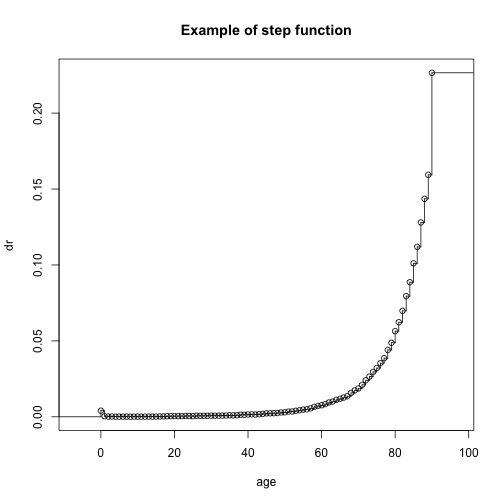
\includegraphics{plot_stepfun-1} \end{center}

We can also initialize a piecewise real function \texttt{f} defined by the function \texttt{dr} before age 80, and by a Gompertz-Makeham intensity function for ages after 80.

\begin{Shaded}
\begin{Highlighting}[]
\NormalTok{f \textless{}{-}}\StringTok{ }\KeywordTok{piecewise\_x}\NormalTok{(}\DecValTok{80}\NormalTok{, }\KeywordTok{list}\NormalTok{(dr, }\KeywordTok{gompertz}\NormalTok{(}\FloatTok{0.00006}\NormalTok{, }\FloatTok{0.085}\NormalTok{)))}
\NormalTok{x \textless{}{-}}\StringTok{ }\KeywordTok{seq}\NormalTok{(}\DecValTok{40}\NormalTok{, }\DecValTok{110}\NormalTok{)}
\KeywordTok{plot}\NormalTok{(x, }\KeywordTok{sapply}\NormalTok{(x, f),}\DataTypeTok{xlab=}\StringTok{"age"}\NormalTok{,}\DataTypeTok{ylab=}\StringTok{"f"}\NormalTok{, }\DataTypeTok{main=}\StringTok{"Example of piecewise function"}\NormalTok{)}
\end{Highlighting}
\end{Shaded}

\begin{center}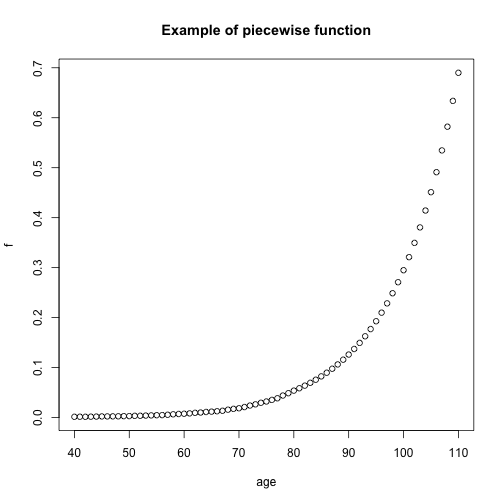
\includegraphics{plot_piecewise-1} \end{center}

\begin{enumerate}
\def\labelenumi{\arabic{enumi}.}
\setcounter{enumi}{1}
\tightlist
\item
  Once a function has been created and defined as model parameter, a model depending on the function can be defined. For example we use in the model below the \texttt{stepfun} \texttt{dr} as a model parameter named \texttt{rate}. The function is used to defined the intensity of death events in the model.
  s
\end{enumerate}

\begin{Shaded}
\begin{Highlighting}[]
\NormalTok{params \textless{}{-}}\StringTok{ }\KeywordTok{list}\NormalTok{(}\StringTok{"rate"}\NormalTok{ =}\StringTok{ }\NormalTok{dr)}
\NormalTok{event \textless{}{-}}\StringTok{ }\KeywordTok{mk\_event\_individual}\NormalTok{(}\StringTok{\textquotesingle{}death\textquotesingle{}}\NormalTok{, }\DataTypeTok{intensity\_code =} \StringTok{\textquotesingle{}result = rate(age(I, t));\textquotesingle{}}\NormalTok{)}
\NormalTok{mod \textless{}{-}}\StringTok{ }\KeywordTok{mk\_model}\NormalTok{(}\KeywordTok{get\_characteristics}\NormalTok{(pop), }\DataTypeTok{events =} \KeywordTok{list}\NormalTok{(}\StringTok{\textquotesingle{}death\textquotesingle{}}\NormalTok{ =}\StringTok{ }\NormalTok{event), }
                \DataTypeTok{parameters =}\NormalTok{ params, }\DataTypeTok{with\_compilation =} \OtherTok{FALSE}\NormalTok{)}
\KeywordTok{summary}\NormalTok{(mod)}
\CommentTok{\#\# Events:}
\CommentTok{\#\# \#1: individual event of type death}
\CommentTok{\#\# {-}{-}{-}{-}{-}{-}{-}{-}{-}{-}{-}{-}{-}{-}{-}{-}{-}{-}{-}{-}{-}{-}{-}{-}{-}{-}{-}{-}{-}{-}{-}{-}{-}{-}{-}{-}{-}{-}{-} }
\CommentTok{\#\# Individual description:}
\CommentTok{\#\# names:  birth death male IMD }
\CommentTok{\#\# R types:  double double logical integer }
\CommentTok{\#\# C types:  double double bool int}
\CommentTok{\#\# {-}{-}{-}{-}{-}{-}{-}{-}{-}{-}{-}{-}{-}{-}{-}{-}{-}{-}{-}{-}{-}{-}{-}{-}{-}{-}{-}{-}{-}{-}{-}{-}{-}{-}{-}{-}{-}{-}{-} }
\CommentTok{\#\# R parameters available in C++ code:}
\CommentTok{\#\# names:  rate }
\CommentTok{\#\# R types:  closure }
\CommentTok{\#\# C types:  function\_x}
\end{Highlighting}
\end{Shaded}

\begin{enumerate}
\def\labelenumi{\arabic{enumi}.}
\setcounter{enumi}{2}
\tightlist
\item
  After compilation, the parameter \texttt{rate} can actually be replaced by any function of type \texttt{function\_x}. For example you can call
\end{enumerate}

\begin{verbatim}
popsim(mod, pop, params = list("rate" = dr), age_max = 120, 
       events_bounds = c('death' = dr(age_max)), time = 10)
\end{verbatim}

as well as

\begin{verbatim}
popsim(mod, pop, params = list("rate" = f), age_max = 120, 
       events_bounds = c('death' = f(age_max)), time = 10)
\end{verbatim}

\hypertarget{piecewise-real-functions-of-two-variables}{%
\paragraph{Piecewise real functions of two variables}\label{piecewise-real-functions-of-two-variables}}

In the C++ code these R functions declared with \texttt{?piecewise\_xy} are identified as \texttt{function\_xy} functions. See \texttt{?piecewise\_xy} for mathematical definition. This function allows to easily define a step function that depend on age and time.

\hypertarget{list-of-functions}{%
\paragraph{List of functions}\label{list-of-functions}}

As parameter you can use a list of functions. All R functions in the list must be of the same C++ type: either \texttt{function\_x} or \texttt{function\_xy}. In C++ code the list of functions is replaced by a \texttt{std::vector} of \texttt{function\_x} or \texttt{function\_xy} (with first element indexed by 0).

\hypertarget{randomvar}{%
\subsection{Random variables}\label{randomvar}}

We use the following notations to describe the available C++ random distributions, which can be used in the C++ intensity and kernel codes.

\begin{itemize}
\item
  \(\mathcal{U}(a,b)\) : Uniform distribution on \([a, b]\) with \(a < b\)
\item
  \(\mathcal{E}(\lambda)\) : Exponential distribution, \(\lambda > 0\)
\item
  \(\mathcal{N}(\mu,\sigma)\) : Gaussian distribution, \(\mu, \sigma \in \mathbf{R}\)
\item
  \(\mathrm{Pois}(\lambda)\): Poisson distribution, \(\lambda > 0\)
\item
  \(\Gamma(\alpha, \beta)\): Gamma distribution, \(\alpha > 0\), \(\beta > 0\)
\item
  \(\mathrm{Weib}(a, b)\): Weibull distribution, \(a > 0\), \(b > 0\)
\item
  \(\mathcal{U}\{a, b\}\): Discrete uniform distribution on \(\{a, a+1, \dots, b\}\) with \(a < b\)
\item
  \(\mathcal{B}(p)\): Bernoulli distribution, the probability of success is \(p \in (0,1)\)
\item
  \(\mathcal{B}(n, p)\): Binomial distribution \(n \ge 1\), \(p \in (0,1)\)
\item
  \(\mathcal{D}_n\) : Discrete distribution with values in \(\{ 0, \dots, n-1 \}\) and with probabilities \(\{p_0, \dots, p_{n-1}\}\).
\end{itemize}

In the table below we show how to call them, which means how to make independent realizations of these random variables, and we give the reference to the C++ corresponding function of the \href{http://www.cplusplus.com/reference/random/}{random library} hidden in this call.

\begin{longtable}[]{@{}lll@{}}
\toprule
Function call & Meaning & C++ \href{http://www.cplusplus.com/reference/random/}{\texttt{random}} internal function\tabularnewline
\midrule
\endhead
CUnif(\(a=0, b=1\)) & \(\mathcal{U}(a,b)\) & \href{http://www.cplusplus.com/reference/random/uniform_real_distribution/}{\texttt{uniform\_real\_distribution\textless{}double\textgreater{}}}\tabularnewline
CExp(\(\lambda=1\)) & \(\mathcal{E}(\lambda)\) & \href{http://www.cplusplus.com/reference/random/exponential_distribution/}{\texttt{exponential\_distribution\textless{}double\textgreater{}}}\tabularnewline
CNorm(\(\mu=0, \sigma=1\)) & \(\mathcal{N}(\mu,\sigma)\) & \href{http://www.cplusplus.com/reference/random/normal_distribution/}{\texttt{normal\_distribution\textless{}double\textgreater{}}}\tabularnewline
CPoisson(\(\lambda=1\)) & \(\mathrm{Pois}(\lambda)\) & \href{http://www.cplusplus.com/reference/random/poisson_distribution/}{\texttt{poisson\_distribution\textless{}double\textgreater{}}}\tabularnewline
CGamma(\(\alpha=1, \beta=1\)) & \(\Gamma(\alpha,\beta)\) & \href{http://www.cplusplus.com/reference/random/gamma_distribution/}{\texttt{gamma\_distribution\textless{}double\textgreater{}}}\tabularnewline
CWeibull(\(a=1\), \(b=1\)) & \(\mathrm{Weib}(a,b)\) & \href{http://www.cplusplus.com/reference/random/weibull_distribution/}{\texttt{weibull\_distribution\textless{}double\textgreater{}}}\tabularnewline
CUnifInt(\(a=0, b=2^{31}-1\)) & \(\mathcal{U}\{a,b\}\) & \href{http://www.cplusplus.com/reference/random/uniform_int_distribution/}{\texttt{uniform\_int\_distribution\textless{}int\textgreater{}}}\tabularnewline
CBern(\(p=0.5\)) & \(\mathcal{B}(p)\) & \href{http://www.cplusplus.com/reference/random/bernoulli_distribution/}{\texttt{bernoulli\_distribution}}\tabularnewline
CBinom(\(n=1, p=0.5\)) & \(\mathcal{B}(n,p)\) & \href{http://www.cplusplus.com/reference/random/binomial_distribution/}{\texttt{binomial\_distribution\textless{}int\textgreater{}}}\tabularnewline
CDiscrete(\texttt{p\_begin}, \texttt{p\_end}) & \(\mathcal{D}_n\) & \href{http://www.cplusplus.com/reference/random/discrete_distribution/}{\texttt{discrete\_distribution\textless{}int\textgreater{}}}\tabularnewline
\bottomrule
\end{longtable}

In the discrete distribution call \texttt{CDiscrete(p\_begin,\ p\_end)}, the arguments \texttt{p\_begin} and \texttt{p\_end} represent the iterators to the begin and to the end of an array which contains \(\{p_0, \dots, p_{n-1}\}\). Note that the use of iterators is a convenient and fast way to access a column or row of a matrix \texttt{arma::mat}.
  </div>

  <div class="col-md-3 hidden-xs hidden-sm" id="pkgdown-sidebar">

        <nav id="toc" data-toggle="toc">
      <h2 data-toc-skip>Contents</h2>
    </nav>
      </div>

</div>



      <footer>
      <div class="copyright">
  <p>Developed by Daphné Giorgi, Sarah Kaakai, Vincent Lemaire.</p>
</div>

<div class="pkgdown">
  <p>Site built with <a href="https://pkgdown.r-lib.org/">pkgdown</a> 1.6.1.</p>
</div>

      </footer>
   </div>

  


  </body>
</html>

